

\chapter{Herstellung und Zusammenbau}
\label{chap:herstllung}

\section{Herstellungsprozess der Komponenten}
\subsection{Skelett und grundlegende Bootsform}
Da für dieses Projekt keine computergesteuerte \ac{cnc} Fräse zur Verfügung steht, werden die Spanten des Bootes mittels einer elektrischen Handstichsäge aus drei verleimten Tannenbrettern mit den Massen 240 mal 40 cm und einer Stärke von 18 mm ausgesägt. Dafür werden die Baupläne der zehn Elemente mithilfe eines Plotters im Massstab 1:1 ausgedruckt und  mit Hilfe von transparentem Backpapier mittels der Abpausmethode auf Tannenholzbretter übertragen, und anschliessend mit der Handstichsäge ausgesägt.

Die Erstellung der Spanten erfolgt in zwei Arbeitsschritten. Im ersten Schritt wird die äussere Form ausgesägt. In einem zweiten Schritt wird danach Material von innerhalb der Elementen entfernt. Dies wird aus Gewichtsgründen gemacht und schafft den für die spätere Montage der Elektronik und der Energieversorgung notwendigen Freiraum im Inneren des Bootes.

An den entsprechenden Stellen an der Oberseite der Elemente werden je zwei Löcher gebohrt und die Elemente werden dann mithilfe zweier Aluminiumstangen ineinander befestigt. Um eine Verschiebung der Elemente während des Herstellungsprozess zu vermeiden wird Heisskleber verwendet. 
\begin{figure}[H]
    \centering
    \includegraphics[width=1\linewidth]{rippe1.png}
    \caption{Rippen förmige Anordnung der Tragelemente}
    \label{fig:enter-label}
\end{figure}

Da die Spanten  mit einer Handstichsäge ausgesägte werden, lassen sich  Ungenauigkeiten nicht völlig vermeiden. Daher weichen die tatsächlichen Masse der Spanten bis zu 5 mm von den Planwerten ab. Obwohl dies eine relative Abweichung ist, kann der Fehler in den folgenden Arbeitsschritten ausgebessert werden. 

Da für die Elemente aus Kostengründen kein Massivholz genommen werden kann, muss auf Leimholz zurück gegriffen werden. Dies hat zum Nachteil, dass einzelne Elemente einen Bruch erleiden, wenn zu viel Druck auf die geleimten Stellen wirkt. Beschädigte Elemente werden nicht verwendet sondern durch neu  erstellt Kopien ersetzt. 
\begin{figure}[H]
    \centering
    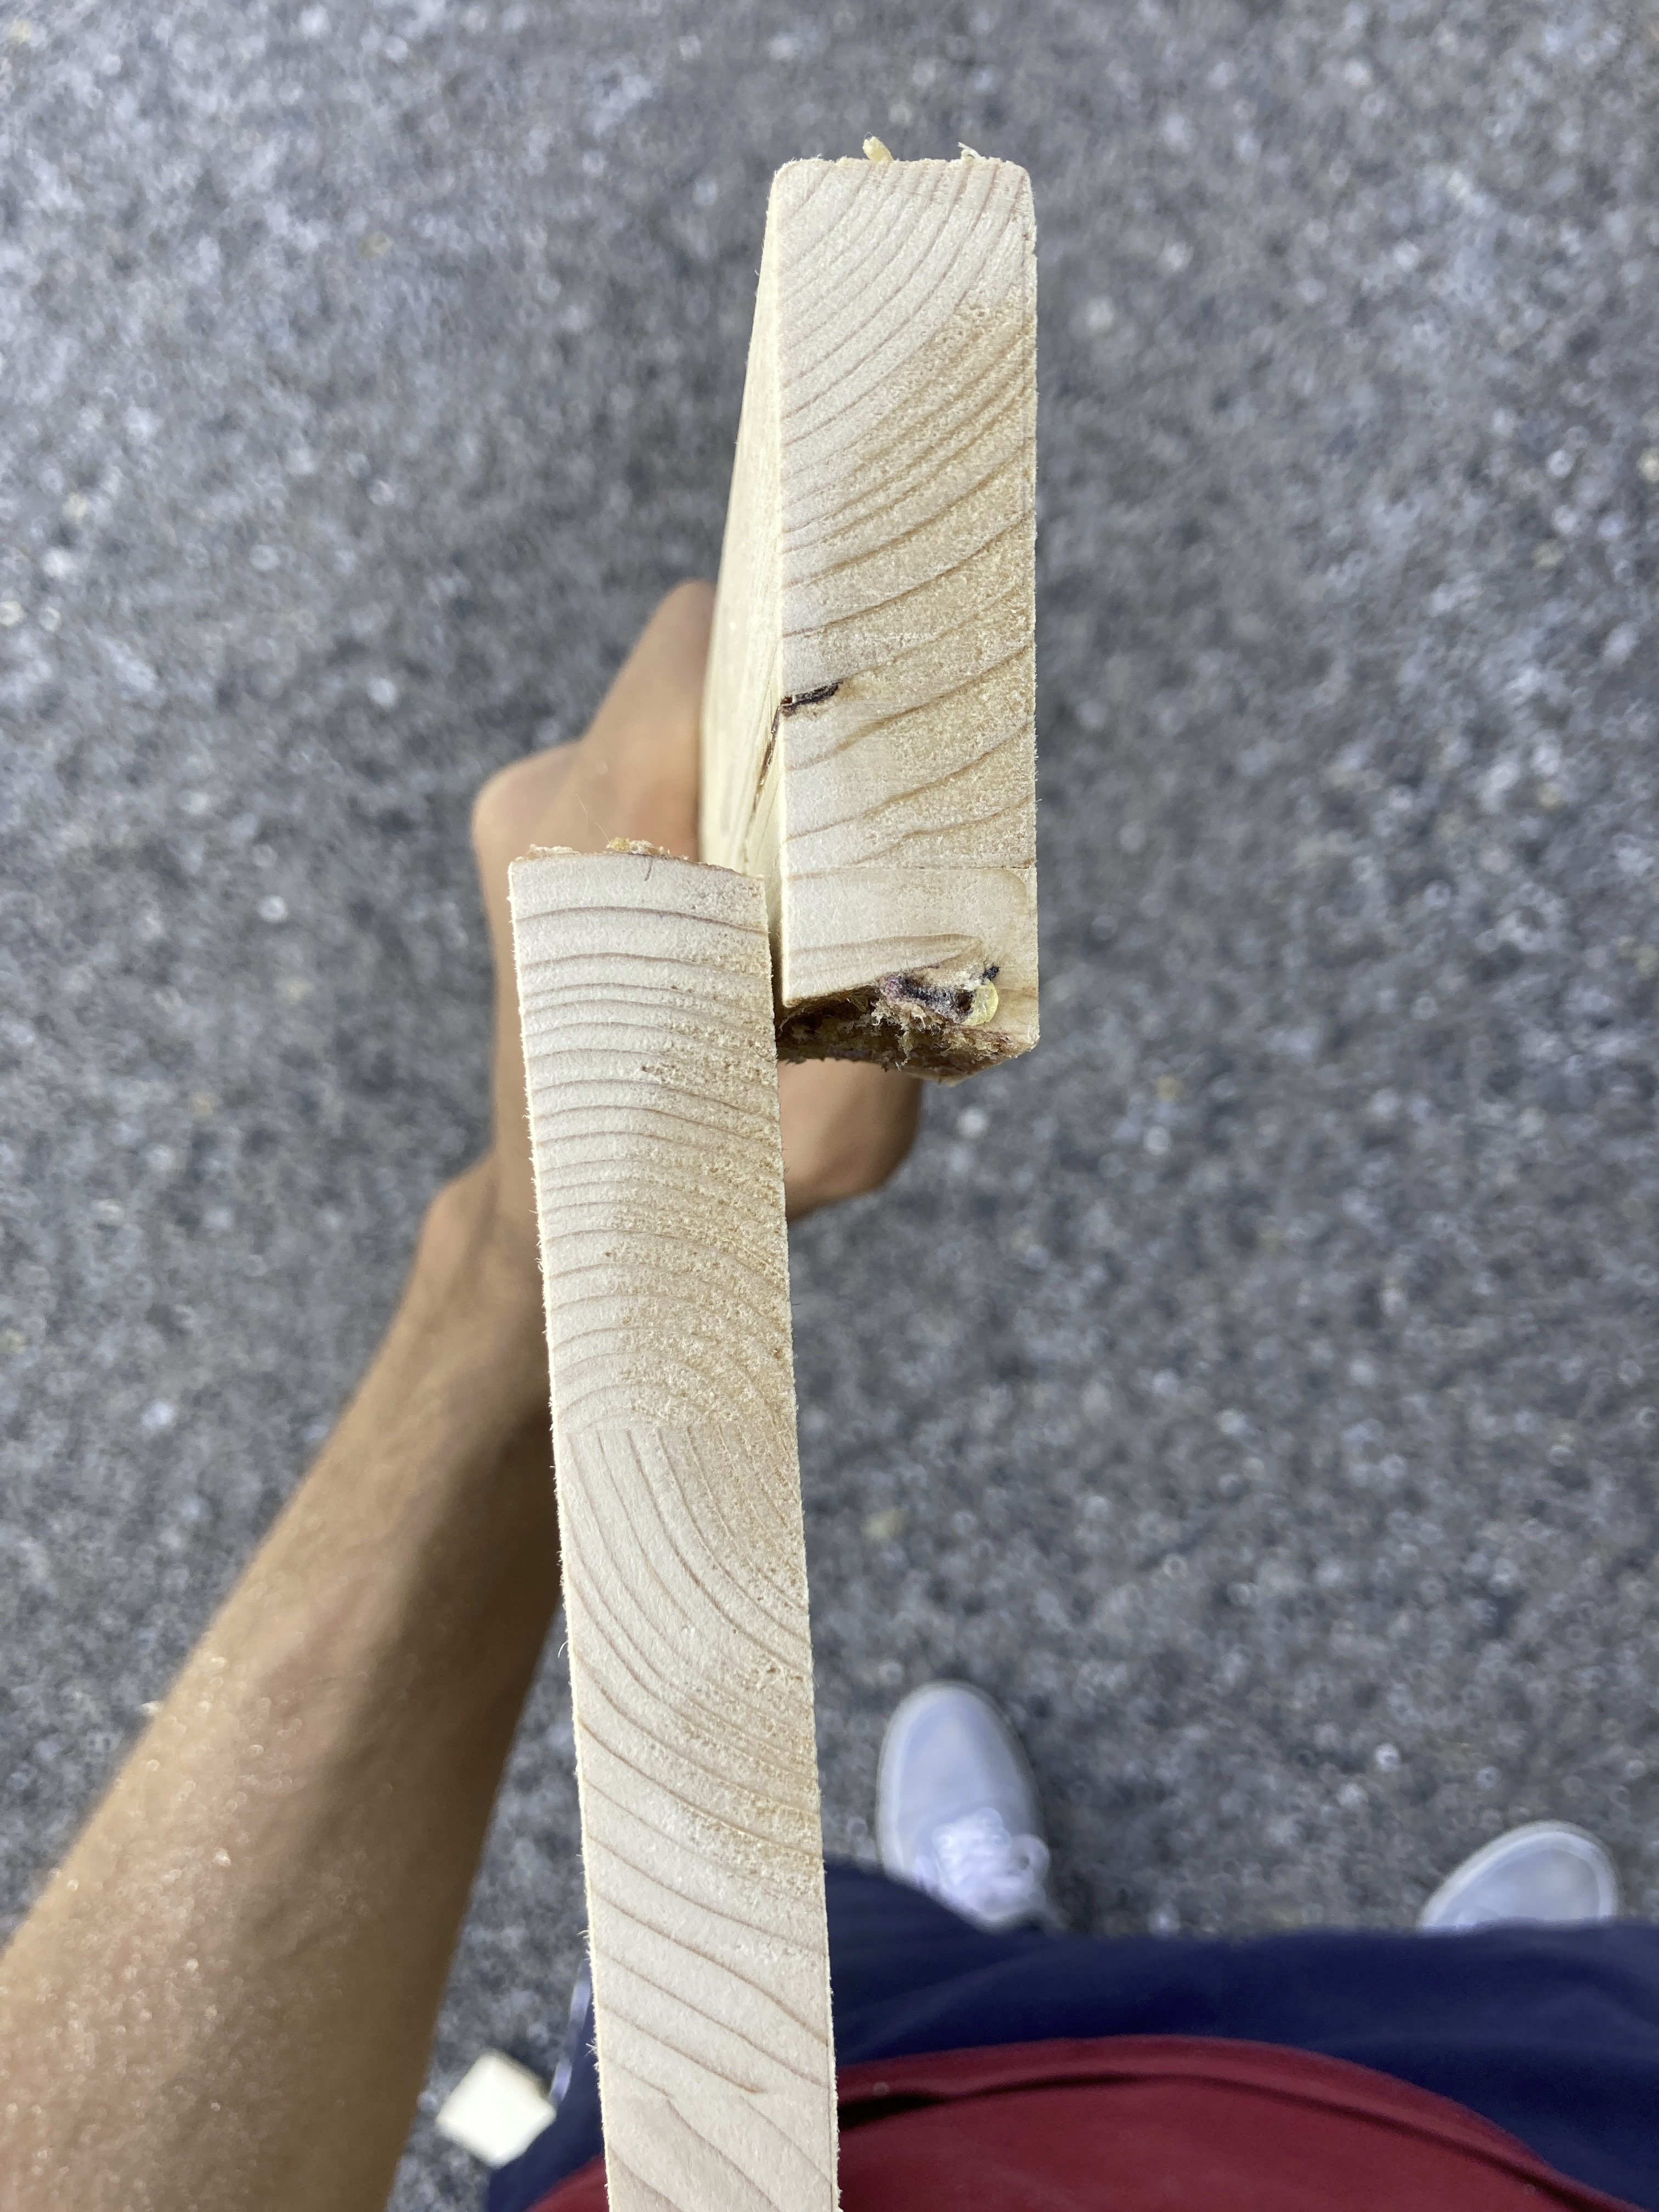
\includegraphics[width=0.25\linewidth]{bruch.png}
    \caption{Bruch eines Elements}
    \label{fig:bruch}
\end{figure}

Im Anschluss wird eine Schicht Balsaholz über die Rippen gelegt. Die verwendeten Balsaholzbrettchen haben eine Stärke von 1mm und sind 100 cm lang. Zur Befestigung an den Spanten wird eine Tackerpistole verwendet. Durch Verspannungen im Holz ergeben sich unglücklicherweise kleinere Verformungen, welche sich negative auf die endgültige Bootsform auswirken können.

\subsection{Glasfaserbeschichtung}
Um eine robuste  Aussejnhülle für das Boot zu schaffen, wird eine glasfaserverstärlte Epoxidharzschicht  aufgetragen. Die Verbndung von Glasfasermatten mit Epoxidharzergibt eine äusserst harte und stabile Schicht.  Dafür  werden die Glasfasermatten auf die Balsaholzplanken gelegt und mit Epoxidharz bestrichen. Dies führt dazu, dass die Epoxidschicht die Form des Bootes animmt. Das unterliegende Balsaholz bildet also  die formgebende, und die Glasfaser-Epoxidschicht die  strukturgebende Komponente. 

Dieses Vorgehen führt jedoch auch zu Problemen, da der Auftrag der Glasfaser-Epoxidschicht zu Verspannungen in der Balsaholzschicht führt. Auch die Schwankungen des Feuchtigkeit in der Werkstatt bewirken Verspannungen, welche sich dann ebenfalls auf die Balsaholzschicht auswirken.  Um diese Dellen in der Auseenhülle auszugleichen, muss sehr viel Expoxidspachtemasse aufgetragen wird. Dafür wird eine Mischung von Expoixid und entsprechendem Härtungsmittel verwendet.  Um das folgende Planschliefen der Oberfläche zu vereinfachen, werden diesem Gemisch Microballons beigemischt und ein Tixotropiermittel wird zugegeben, um das Gemisch einzudicken. Der Prozess des Auftragens und Abschliefens muss  viele Male wiederholt werden. Das ist sehr zeitaufwändig, da immer gewartet werden muss, bis die neu aufgeragenene Schicht vollständig ausgetroknet ist.  Dabei wird  versucht wird einen möglichst glatten, stromlinienförmigen Körper zu formen.

Um eine Asymetrie beim Bug zu vermeiden, wird sehr viel Expoxid-Spachtelmasse augetragen. Kleine Glasfaserschnippsel, welche zu Spachtelmasse dazugerührt werden, geben dieser weitere Stabilität, damit der Bug gut geschützt ist.
\subsection{Ruder}
Das Ruder wird aus einer Tannen-Leimholz Platte ausgesägt. Dabei wird daselbe Verfahren wie bei den Spanten angewendet. Anschliessend wird das Werkstück mit der Schliefmaschine bearbeitet und in Form gebracht. 

Nach der Lackierung mit roter Farbe wird das Ruder am Heck des Schiffskörpers befestigt und mit der Welle des Aktuators verbunden.
\subsection{Kiel}
In einem ersten Schritt werden die 5 Bretter ausgesägt, mit einander verleimt und verschraubt. Anschliessend werden in die Löcher für die Gewindestangen in die beiden äusseren Kielbretter gebohrt. 

Im nächsten Schritt wird ein Loch in die beiden 2 Kg Gewichte gebohrt. So können die Gewichte mit dem Kielhauptbrett verschraubt werden. Nach dem Druck der beiden Schutzgehäuse werden diese über die Gewichte gestülpt und mit dem Kielhauptbrett verleimt.    
\begin{figure} [H]
    \centering
    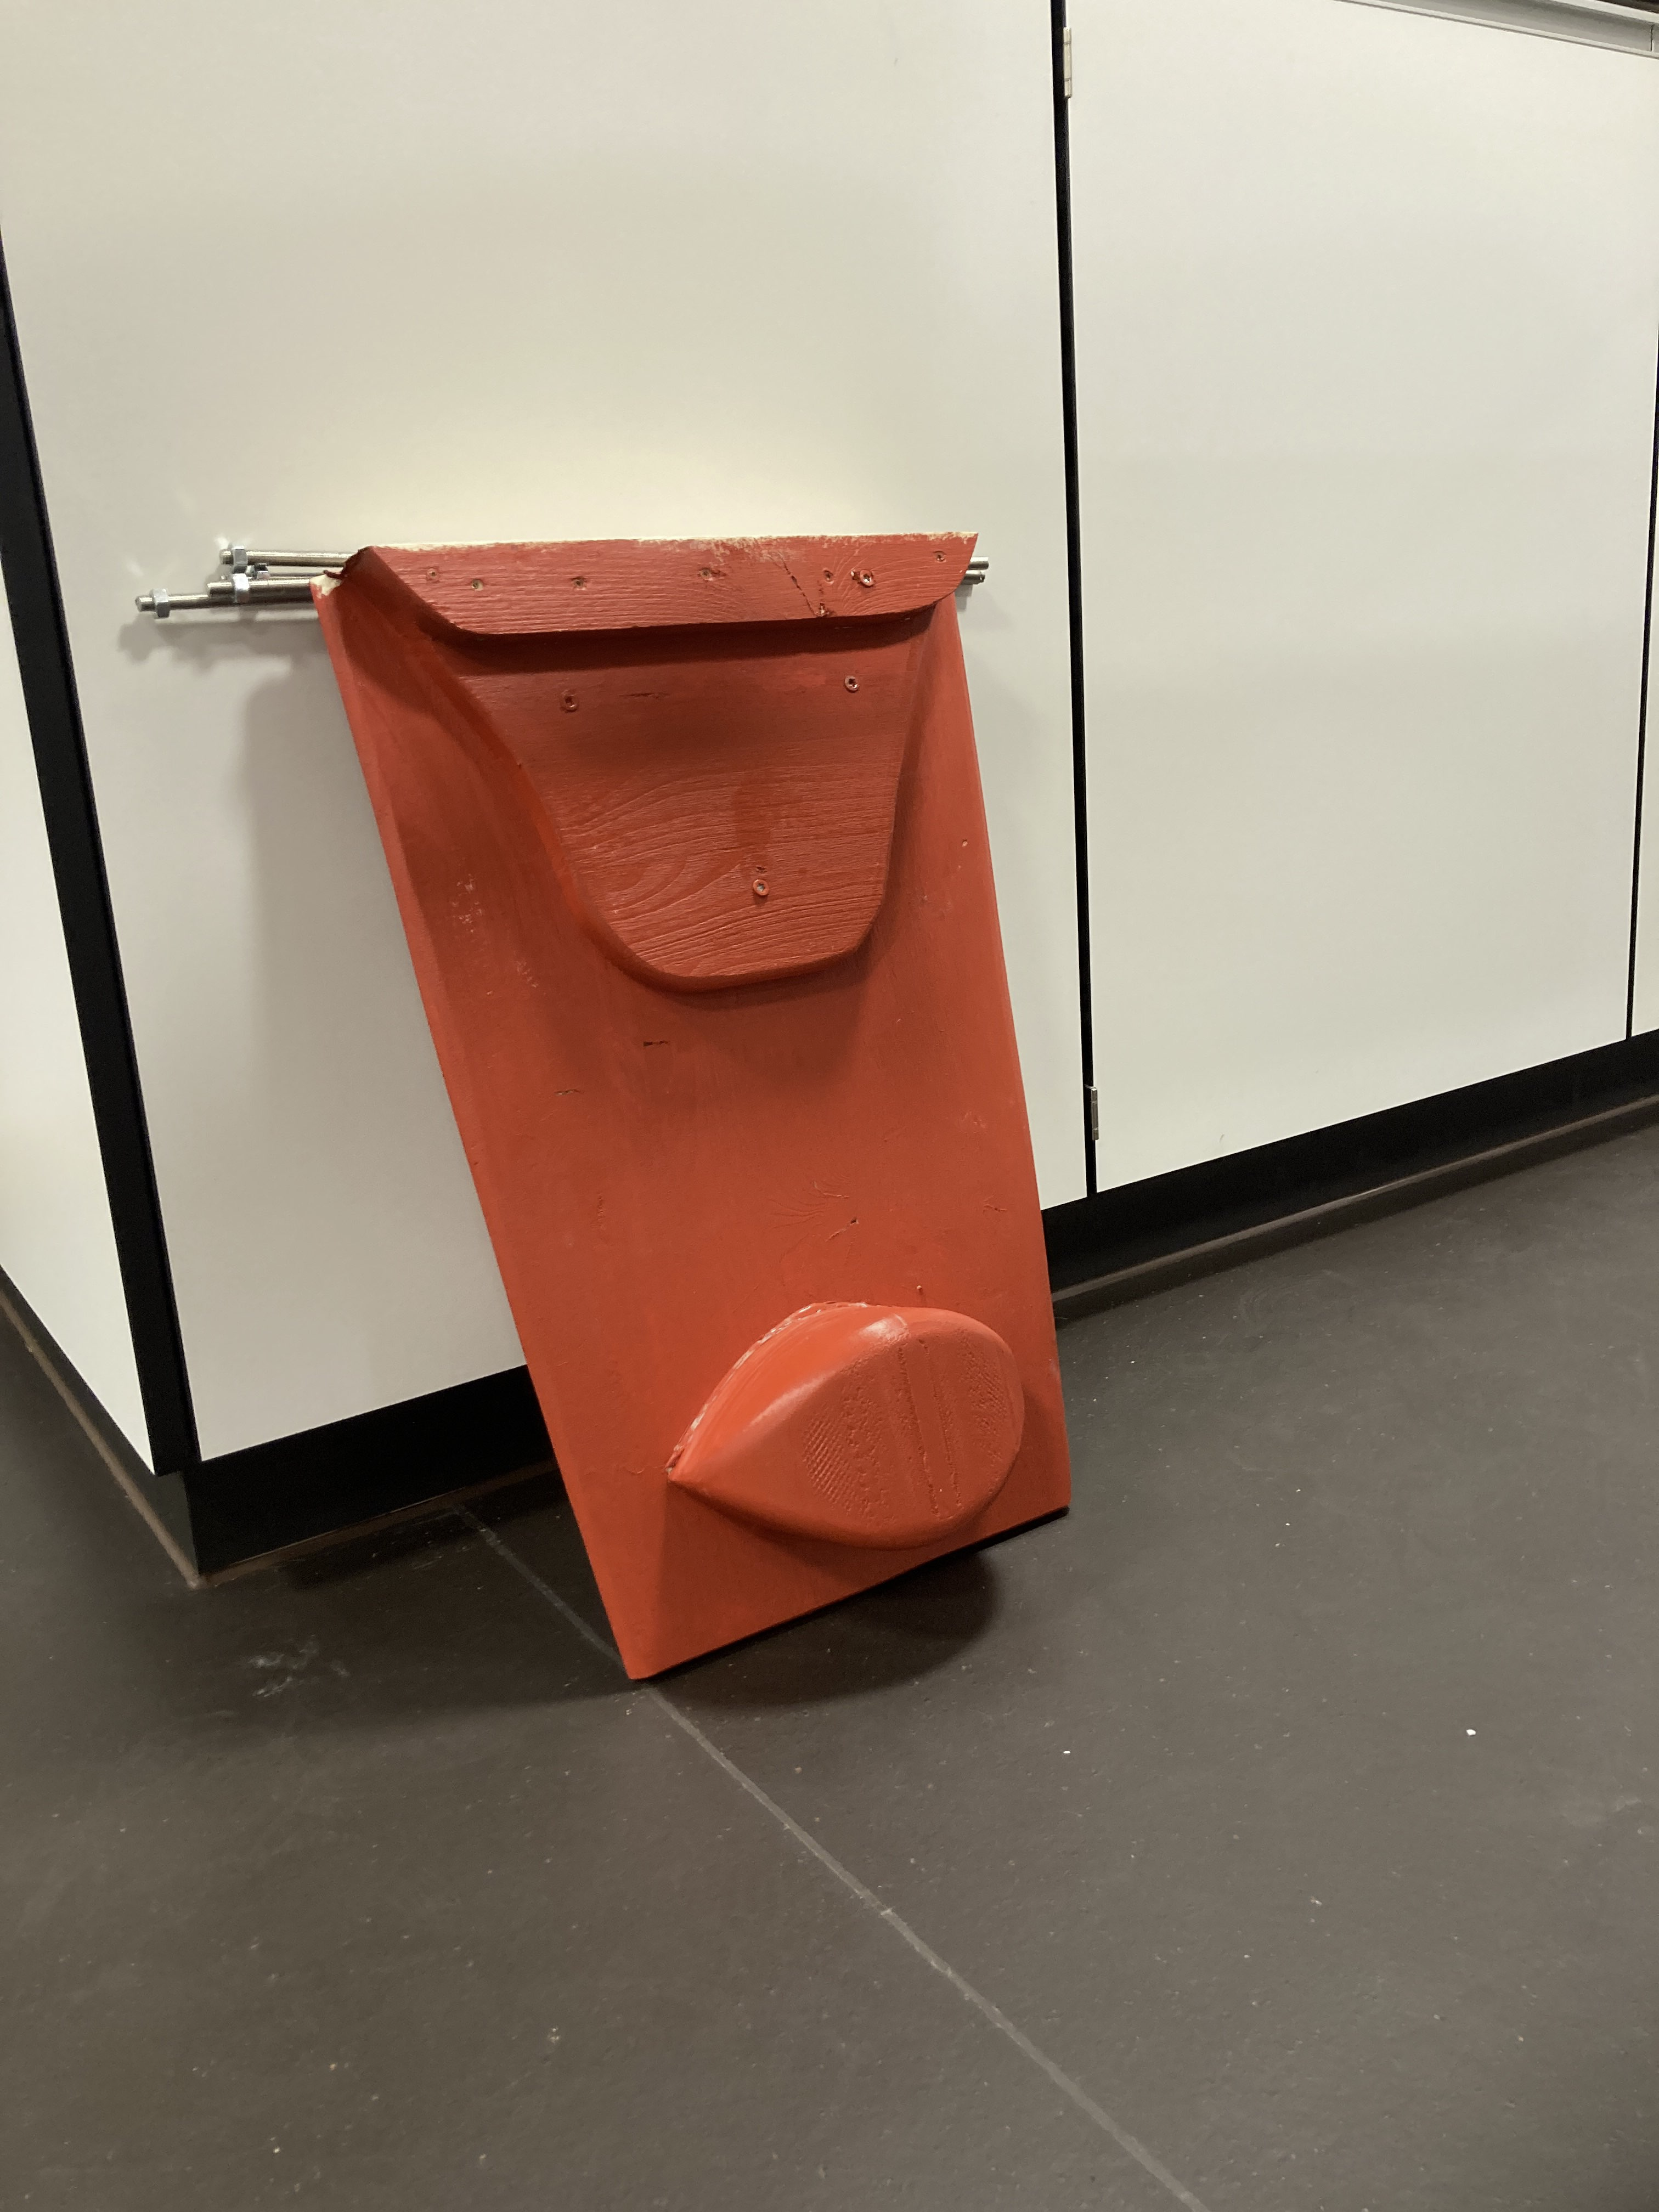
\includegraphics[width=0.3\linewidth]{assets/Kiel_lakiert.png}
    \caption{Fertiger Kiel}
    \label{fig:enter-label}
\end{figure}

\subsection{Segel}
Das Segel besteht aus EPS und setzt sich aus vier identischen Teilen zusammen, die aus EPS-Platten ausgeschnitten werden. Je zwei Platten bilden die rechte und die linke Seite des Segels, das eine aerodynamisch günstige Form aufweist. Dazu werden die beiden Segelhälften verklebt.  
\subsubsection*{EPS Schneidgerät}
Mit speziellen Schneideräten können Formen aus EPS Platten geschnitten werden. Konventionelle EPS Schneidgeräte sind allerdings nicht genügend gross, um dien vier Teile auszuschneiden, weshalb ein eigenes Schneidgerät gebaut werden muss. Alle EPS Schneidegeräte funktionieren nach demselben Prinzip. Dabei wird ein Metalldraht  auf  60$^\circ$ C - 100$^\circ$ C) erhitzt und ins EPS gefahren, wo dieses lokal zum Schmelzen gebracht wird. Indem der Draht durch den EPS Körper gezogen wird, entsteht damit ein sauberer Schnitt. Der Draht wird dadurch erhitzt, dass an ihn eine elektrische Spannung gelegt wird. Der Draht bildet einen Widerstand und wird hiess.. Der Draht ist so ausgelegt, dass er einen möglichst hohen Wiederstand aufweisst. 

Damit die  vier grossen Segelteile als ganzes aus EPS Blöcken geschnitten werden können, wird ein eigenes einfaches Schneidegerät mit entsprechenden Dimensionen gebaut.  Dazu wird ein sogenannter \enquote{Wiederstandsdraht} mit einem Durchmesser von $\varnothing$ 0.2mm gekauft. Dieser wird dreifach Verdrillt und daraus ein Schneidedraht mit einer Länge von 1.5 m erstellt. Die beiden Enden werden in einen U-förmigen Rahmen aus Tannenholzlatten gespannt. Als Stromquelle dient zunächst ein Labornetzteil, das 3A bei 12V liefert. 

Die ersten Versuche, zunächst noch mit einem einfache, und anschliessend mit einem zweifachen Draht verlaufen erfolglos. Erst als eine dreifach verdrillter Draht und ein stärkeres Labornetzteil, das 5A bei 12 V liefert, verwendet werden, wird der Draht soweit aufgeheizt, dass damit EPS geschnitten werden kann.     


\begin{figure}[H]
    \centering
    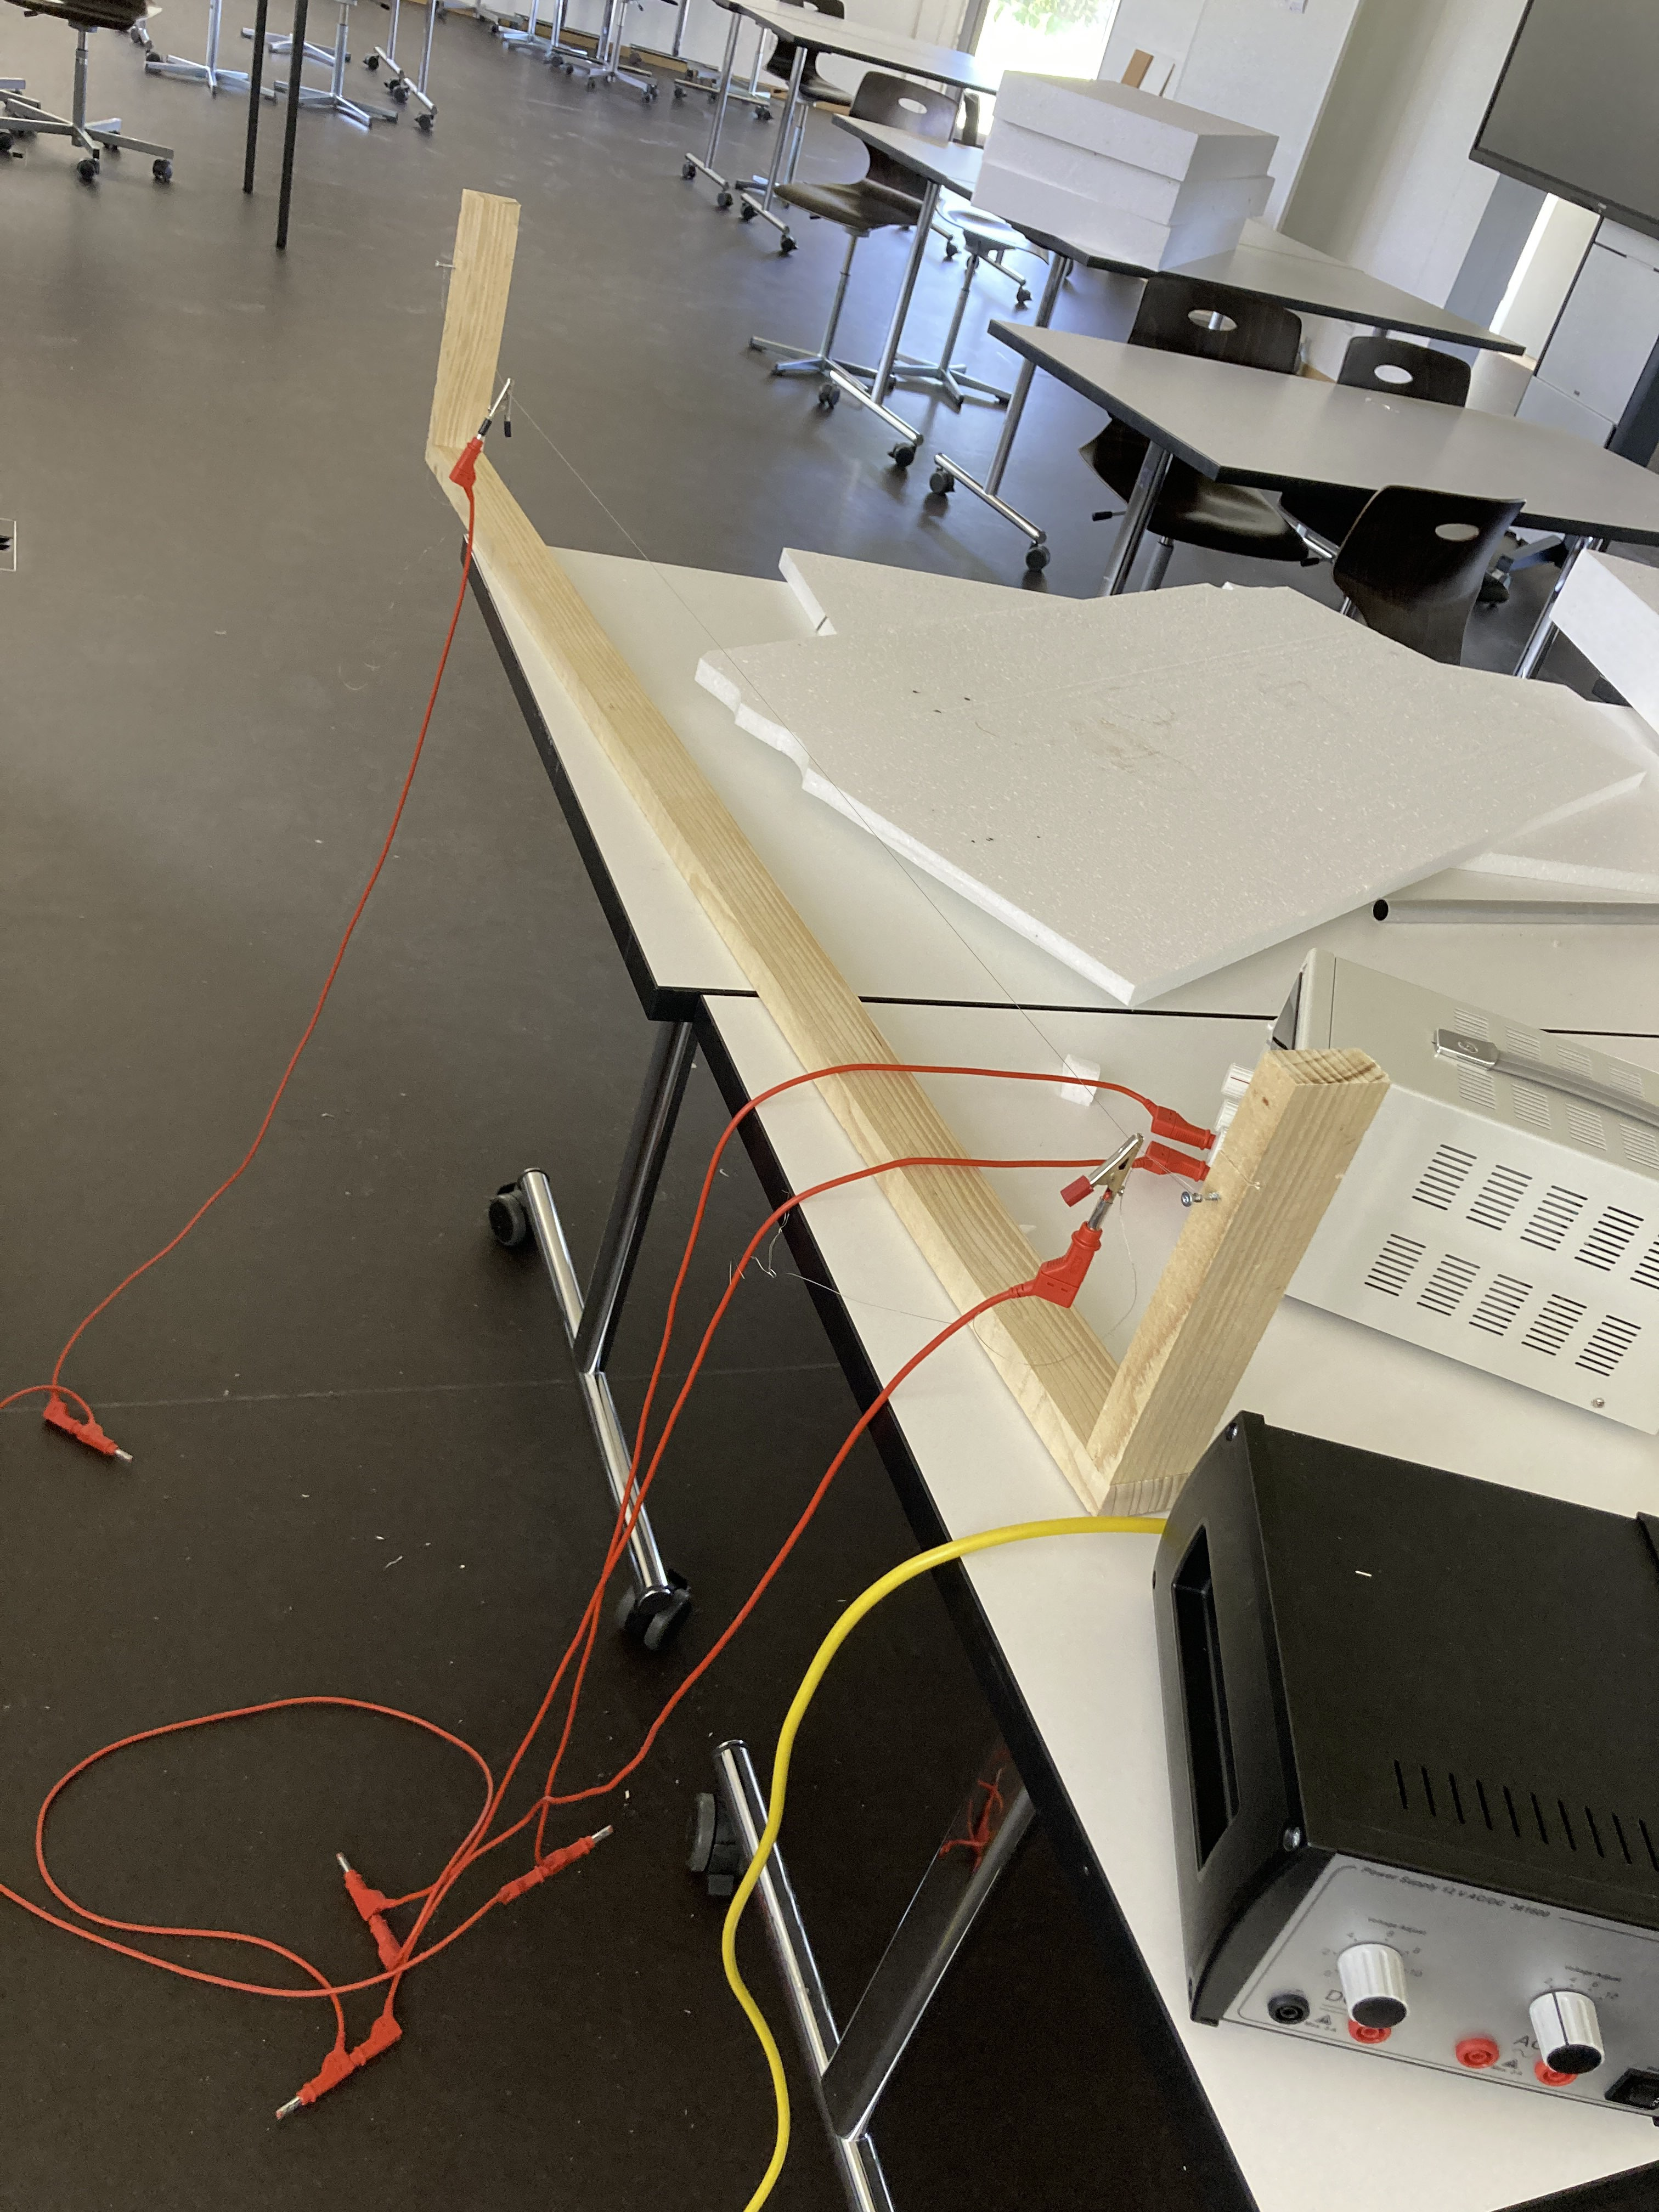
\includegraphics[width=0.5\linewidth]{foamcutter1.png}
    \caption{Foamcutter}
    \label{fig:enter-label}
\end{figure}

\subsubsection*{Grosssegel}
Um die geplante Form aus den \ac{eps} Platten schneiden zu können, wird zuerst mithilfe eines Lasercutters eine Halbprofilform aus Sperrholz erstellt. Je eine solche Halbprofilform wird mit zwei  Schraube an den beiden kürzeren Seiten einer EPS Platte  befestigt . Der heisse Schneidedraht kann damit entlang der Kante der Halbprofilschablone durch den EPS Block gezogen werden. So entsteht ein halbes Segel mit der Form der Halbprofilschablonen . \\


\begin{figure}[H]
    \centering
    \includegraphics[width=1\linewidth]{assets/template_on_foam.png}
    \caption{Seitenansicht eines Elements mit der Schablone}
    \label{fig:enter-label}
\end{figure}

Anschliessed muss auf der planen Seite des Halbsegelteils noch eine halbrunde Kerbe ausgeschnitten werden. In ihr findet bei der Verleimung der Platten der Aluminiummast platz. Nicht jeder Schneidversuch verläuft erfolgreich. Wenn die beiden Enden des Schneiddrahtes nicht synchron über die Halbprofilform geführt werden, oder wenn dieser nicht präzis gefolgt wird, weist der ausgeschnittene Körper erhebliche Formfehler auf. Auch bei einem an sich erfolgreichen Schnitt ergeben sich aber kleine Ungenauigkeiten, die aber mit einem Schliff des Bauteils korrigiert werden können. 

Nachdem erfolgreich vier Profile ausgeschnitten worden sind, wird der Mast in die ausgesparte Kerbe gelegt und fixiert. Danach werden die vier Profile in Paaren verklebt.      

\subsection{Saailflap}
Das Sailflap wird mit der selben Technik wie das Grosssegel hergestellt. Es wird mit zwei Carbonstäben am Grossselgel fixiert. In einem letzten Schritt wird der Aktuator ins Grosssegtel einbebaut und mit dem Sailflap verbunden.   
\section{Bemalung}
Da das autonome Segelboot gut sichtbar sein soll, wird es in roter Signalfarbe bemalt. Dazu wird seidenmatter Acryllack verwendet, der mithilfe einer Farbwalze auf den Bootskörper aufgetragen wird. Es wurde bewusst  eine matte Farbe  gewählt, da diese kleine Ungenauigkeiten und Dellen in der Bootsform besser kachiert als glänzende Farben. 

Da das Rudern, der Kiel und das Deck keine Schützhülle aus glasfaserverstärktem Epoxidharz verfügen, dient hat die Farmlackierung bei diesen Bauteilen auch eine Schutzfunktion.
\section{Einbau der Elektronik}
Als erstes wird ein digitaler Schaltplan mit allen Sensoren und Aktuatoren und Sensoren erstellt. Dieser dientals Bauanleitung für den Bau. Die für die Erstellung des Schaltplan notwendigen Informationen werden den Datenblättern der Geräte und  Sensoren entnommen, in denen ihre Funktionsweise beschrieben und die Betriebsweise erläutert werden.
\subsection{Raspberry Pi}
Der Raspberry Pi Zero W 1.1 wird direkt über seinen 5V Pin angesteuert. Zwischen den Energiespeicher und dem Rapberry Pi iZero W 1.1 wird ein Spannungswandler geschaltet, der die ca. 7V Ausgangsspannung des Energiespeichers auf 5V reduziert.

Diese Vorgehensweise hat den Nachteil, dass dass der Raspberry die gesamte Schutzelektronik, welche beim USB Port angebracht ist, überspringt. Der bedeutende Vorteil ist jedoch, dass verlötete Verbindungen  permanent sind und diese sich ohne erhbeliche Gewalt bei Normaltemperaturen nicht lösen. Bei einem sich durchgehend bewegten System ist dies notwenig. 

Ein Ausfall der Bordelektronik würde für das Boot katastrophal enden. 
\subsection{Aktuatoren}
Wie im Kapitel \enquote{Elektronik} bereits erläutert, verfügen die verwendetet Aktuatoren über 3 pins. V+, GND und einen Datapin. 

Da der Raspberry Pi Zero W 1.1 über seine 5V output pins nicht genügend Leistung für das Ansteuern eines, und schon gar nicht von den mehrerer Aktuatoren verfügt, werden diese direkt mit dem Stromversorgung verbunden. Da die Geräte über eine gemeinsamen Groundleitung \enquote{common Ground} verfügen, kann der Raspberry Pi Zero W 1.1 den Aktuator dennoch ansteuern. 

Ein weiteres Problem ergibt sich daraus, dass an den Datenpins des Raspberry Pi Zero W 1.1 nur Steuersignale von 3.3V ausgegeben werden, der Aktuator aber ein 5V Steuersignal benötigt. Der Aktuator kann damit nicht direkt vom Raspberry Pi Zero W 1.1 ansteuert werden. Dieses Problem lässt sich aber einfach  ösen, indem ein Pegelumsetzer zwischengeschaltet werden. 